% BrokerGuard v3 -- Springer LNCS.
% ENGLISH VERSION (2026-11-19). Same structure, tables, figures and numbers as the Vietnamese reading draft in ../latex/.
% Every number comes from ../../iccies2027/facts.md (Test-4 sections, the 19/11 supplements and "Bổ sung cho bài v3").
% British spelling. No first person ("this paper", passive voice, or the system as subject).
% Overleaf: upload the whole latex_en/ folder (zip), main = main.tex, pdfLaTeX. Figures 1--3 are TikZ/pgfplots code.
% Check the venue's policy on AI-generated text before submission and revise the prose in the authors' own words.
\documentclass[runningheads]{llncs}

% T5 (not T1): Section 4 quotes Vietnamese cue words (e.g. ``đừng gửi''), whose letters exist only in T5. English text is
% unaffected. If T5 fonts fail, switch to XeLaTeX: \usepackage{fontspec} \usepackage[english]{babel}.
\usepackage[T5]{fontenc}
\usepackage[utf8]{inputenc}
\usepackage[english]{babel}
\usepackage{graphicx}
\usepackage{booktabs}
\usepackage{multirow}
\usepackage{amsmath,amssymb}
\usepackage{xcolor}
\usepackage{url}
\usepackage{adjustbox}   % max width=\textwidth: figures and tables never exceed the margins
\usepackage{tabularx}
\usepackage{makecell}
\usepackage[section]{placeins}
\usepackage{pgfplots}
\pgfplotsset{compat=1.18}
\usetikzlibrary{patterns,arrows.meta}
% Colour-blind-checked categorical pair (blue/orange). Orange = BrokerGuard (new components), blue = BG-Base,
% grey = other defences. Colour follows the entity in every figure.
\definecolor{bgblue}{HTML}{2A78D6}
\definecolor{bgorange}{HTML}{EB6834}
% Extra stretch so that monospaced words (tool names, e-mail addresses) never stick into the right margin
\setlength{\emergencystretch}{3em}
\usepackage{enumitem}
\setlist{noitemsep, topsep=2pt}

% Floats near their first mention, less white space (LNCS margins, font size and spacing unchanged)
\renewcommand{\topfraction}{0.85}
\renewcommand{\textfraction}{0.1}
\renewcommand{\floatpagefraction}{0.75}
\setcounter{topnumber}{3}
\setcounter{totalnumber}{4}
\setlength{\textfloatsep}{8pt plus 2pt minus 2pt}
\setlength{\floatsep}{6pt plus 2pt minus 2pt}
\setlength{\intextsep}{6pt plus 2pt minus 2pt}
\makeatletter
\setlength{\@fptop}{0pt}
\setlength{\@fpsep}{10pt plus 2pt}
\setlength{\@fpbot}{0pt plus 1fil}
\g@addto@macro\normalsize{%
  \setlength{\abovedisplayskip}{4pt plus 2pt minus 1pt}%
  \setlength{\belowdisplayskip}{4pt plus 2pt minus 1pt}%
  \setlength{\abovedisplayshortskip}{2pt plus 1pt}%
  \setlength{\belowdisplayshortskip}{2pt plus 1pt}}
\makeatother

% Author notes; remove before submission.
\newcommand{\todo}[1]{\textcolor{red}{[TODO: #1]}}
\newcommand{\code}[1]{\texttt{#1}}

% ---- NAMES (change one line to rename throughout; mapping to the logs in ../README.md) -----------------
% A brand-new paper: no version names (v1, v2, v3, BG-Base, Test-I/II/III). Codes only where needed: C1--C3 in their
% definitions, tables and figures; H1--H4, (A1)--(A5), (G1)--(G4) for the tests and proofs; mechanism codes only in
% tables and figures. Prose uses full names. Each name has a mid-sentence form and a capitalised form.
\newcommand{\ours}{\textsc{BrokerGuard}}     % V3P2 (log: v3)
\newcommand{\strSand}{string rules + Sandwich} % D2P2 (log: v1, final_config_v3) = BrokerGuard without C1, C2, C3
\newcommand{\StrSand}{String rules + Sandwich}
\newcommand{\strRules}{string rules}         % D2 = string rules + Sandwich without the prompt layer
\newcommand{\StrRules}{String rules}
\newcommand{\phrRules}{phrase rules}         % R1
\newcommand{\PhrRules}{Phrase rules}
\newcommand{\noDef}{no defence}              % A0
\newcommand{\NoDef}{No defence}
\newcommand{\cSpot}{Spotlight}               % P1
\newcommand{\cSand}{Sandwich}                % P2
\newcommand{\cPG}{PromptGuard}               % G1 (Prompt Guard 2, 86M)
\newcommand{\cMel}{MELON$^*$}                % MEL (re-implementation)
\newcommand{\cProg}{Progent$^*$}             % PRG (re-implementation)
% The three components: names in prose, codes in tables and figures
\newcommand{\pOne}{intent policy}            % C1
\newcommand{\pTwo}{value-level labelling}    % C2
\newcommand{\pThree}{parameter pinning}      % C3
\newcommand{\POne}{Intent policy}
\newcommand{\PTwo}{Value-level labelling}
\newcommand{\PThree}{Parameter pinning}
\newcommand{\cOne}{\textsf{C1}}
\newcommand{\cTwo}{\textsf{C2}}
\newcommand{\cThree}{\textsf{C3}}
% Base rules at the broker (no R-... codes)
\newcommand{\rDest}{substring destination rule}    % D2 rule 2, replaced by C1
\newcommand{\rFlow}{source-label flow rule}        % D2 rule 3
\newcommand{\rRedact}{answer redaction rule}       % D2 rule 4
\newcommand{\rSig}{injection-signal rule}          % D2 A1 layer
\newcommand{\Rdest}{Substring destination rule}
\newcommand{\Rflow}{Source-label flow rule}
\newcommand{\Rredact}{Answer redaction rule}
\newcommand{\Rsig}{Injection-signal rule}
% Attack mechanisms (tables and figures only)
\newcommand{\mER}{\textsf{ER}}               % M1 explicit redirection
\newcommand{\mCR}{\textsf{CR}}               % M2 covert redirection
\newcommand{\mSL}{\textsf{SL}}               % M3 sink leakage
\newcommand{\mAL}{\textsf{AL}}               % M4 answer leakage
\newcommand{\mPT}{\textsf{PT}}               % M5 parameter tampering
\newcommand{\mUS}{\textsf{US}}               % M6 unrequested side effect
% Data sets (use with an article: "the \dev")
\newcommand{\dev}{development set}           % Dev v4.1 (168 families)
\newcommand{\test}{test set}                 % Test-4 (T5_*), the only held-out test set of this paper
% Notation
\newcommand{\sub}{\sqsubseteq}               % x ⊑ z: kappa(x) is a substring of kappa(z)
\newcommand{\dest}{\mathit{dst}}
\newcommand{\data}{\mathit{data}}
\newcommand{\norm}{\nu}
\newcommand{\bPlain}{plain benign}           % benign_plain
\newcommand{\bAuth}{authorised benign}       % benign_auth

% hyperref last: citations, cross-references, DOIs and URLs in blue and clickable
\usepackage{hyperref}
\definecolor{linkblue}{HTML}{1F4E9A}
\hypersetup{colorlinks=true, linkcolor=linkblue, citecolor=linkblue, urlcolor=linkblue}
\AtBeginDocument{\def\doi#1{\href{https://doi.org/#1}{doi:#1}}}

\begin{document}

\title{BrokerGuard: Intent-Aware Authorisation and Value-Level Flow Control Against Indirect Prompt Injection in
Vietnamese LLM Agents}
\titlerunning{BrokerGuard}

\author{\todo{Author 1}\inst{1} \and \todo{Author 2}\inst{1}}
\authorrunning{\todo{Author} et al.}
\institute{\todo{Affiliation, city, country} \\ \email{\todo{email}}}

\maketitle

% LNCS: abstract 150--250 words. No p-values in the abstract. Numbers: facts.md (Test-4: 40, 6, 2 families; ΔU −3.1;
% H1 not significant; tokens and latency of v3 against v1), adaptive rounds, AgentDojo v3.
% 15-page version (2026-11-20), condensed from the long version in commit 6814b3a.
% 20/11: synchronised with the Vietnamese version after owner feedback (round 1 and language pass).
% 20/11 (round 3b, English only): wording and connectives pass, Figure 2 on with [H].
% 20/11 (round 3c): notation only where equations need it, the request in words elsewhere, gate conditions as a list, plainer claims.
\begin{abstract}
Instructions planted in content that an LLM agent reads through its tools can make the agent send data to an unknown
destination, leak confidential values or alter a legitimate action. This paper proposes \ours, a deterministic
policy-enforcement mechanism at the Tool Broker that combines three components without any extra LLM call: an intent
policy that is extracted from the user request and handles negation, sensitivity labels for individual values, and
pinning of the values the user stated. Authorisation safety, confidentiality and integrity are proved on a
state-transition model under five explicit assumptions. On a Vietnamese test set of 48 attack families, sealed before
any code was written, \ours{} reduces the number of harmed families on three open-weight backbones from 40 with no
defence to 2. With string-matching rules in place of the three components, 6 families remain harmed. \ours{} blocks four
of these, each with the component designed for it, lets no new family through, and shows the same direction on every
backbone. Because string matching is already near the floor, confirming this difference with the pre-registered test
requires a larger test set. Utility drops by 3.1 percentage points relative to no defence, and tokens and latency
stay within 1.4\% of string matching. In two rounds of adaptive attacks, no family succeeds that does not already
succeed with the original attack. On AgentDojo in English and Vietnamese, attack success stays low, at the cost of
utility on tasks whose destinations come from tool data.

\keywords{Indirect prompt injection \and LLM agents \and Intent-based authorisation \and Information flow control \and
Vietnamese}
\end{abstract}


% Numbers: facts.md (Test v3 and Test-3: 32.9 -> 1.2%, 32.4 -> 3.8%; the 40 v1 bypasses by cause, section "Bổ sung sau
% phản biện 3"; broker micro-benchmark, section "Bổ sung cho bài v3"). A brand-new paper: the early stage (string rules on
% two sealed sets) is described as part of this study, not as a previous version.
\section{Introduction}\label{sec:intro}

In the ReAct paradigm~\cite{yao2023react}, an LLM agent interleaves reasoning with tool calls such as document search,
database queries or sending e-mail. Whatever a tool returns enters the context of the model directly. In indirect prompt
injection~\cite{greshake2023indirect}, an attacker plants instructions in third-party content that the agent will read.
If the model follows them, the agent may send data to an unknown destination, leak a confidential value or alter
content that the user asked it to send. Prompt-level defences depend on whether the model complies, and injection
classifiers are mostly trained and evaluated on English. Another line of work enforces policy on the host side, between
the model and the tools, following the reference-monitor principle~\cite{anderson1972}.

The simplest way to enforce policy at the Tool Broker is string matching. The broker executes an outgoing call only if
its destination occurs as a substring of the user request $u$, and lets a value taken from a source labelled
confidential leave the agent only if $u$ contains that value verbatim. In the early stage of this study, such
string-matching rules, combined with sandwich prompting, were evaluated on two sealed Vietnamese test sets with three
open backbones. The attack success rate fell from 32.9\% to 1.2\% on the first set and from 32.4\% to 3.8\% on the
second. An analysis of all 40 remaining successful attacks reveals three gaps (Table~\ref{tab:mechanisms}). In 25 cases
a confidential value leaked from a source labelled public, because labels are attached to whole sources rather than to
individual values. In 5 cases the call went to a destination that appears in $u$ but was not authorised, for example one
named in a prohibition. The remaining ten cases altered a parameter of a call to a legitimate destination. These cases
show that the presence of a string in $u$ does not amount to an authorisation, and that the label of a source does not
determine the sensitivity of each value it contains.

This paper proposes \ours, an enforcement mechanism at the broker with three deterministic components. The intent
policy replaces the substring destination rule. It extracts structured grants from $u$, takes the scope of negation and
exclusion into account in Vietnamese and English, and authorises only destinations that match a whole token. Value-level
labelling assigns a sensitivity to each value in tool outputs by the type of the value, independently of the source
label, and checks the flow of these values to every sink and to the final answer. Parameter pinning makes an authorised
call keep the values that the user stated. The policy is derived from $u$ alone, never from tool content, and does not
rely on the judgement of an LLM. When authority is unclear, the result is \emph{needs confirmation}. The two test sets of
the early stage were used to design these components, so they were merged into the development set, and \ours{} is
evaluated on a new test set.

The paper makes three main contributions.
\begin{enumerate}
\item \textbf{Method.} \ours{} closes the three measured gaps of string-matching rules without extra LLM calls. The
  broker check takes less than a millisecond per call (Section~\ref{sec:method}).
\item \textbf{Formal model.} The broker is specified as a state-transition system. Three propositions on authorisation
  safety, confidentiality and integrity are proved under five assumptions. The paper separates the properties that are
  proved from those that are only tested empirically (Section~\ref{sec:formal}).
\item \textbf{Evaluation.} \ours{} is frozen on the development set and run once on a test set of 48 new attack
  families, sealed before any \ours{} code was written, with pre-registered hypotheses. The evaluation compares \ours{}
  with published defences and with simpler rule configurations at the broker, and covers per-component ablations, two
  rounds of adaptive attacks, token and latency costs, the trade-off between security and utility, AgentDojo in English
  and Vietnamese, and a reference column with a closed model (Sections~\ref{sec:protocol} and~\ref{sec:results}). The
  primary hypothesis is not statistically significant, and Section~\ref{sec:discussion} analyses why.
\end{enumerate}
Data, code and the sealing manifests are publicly released.

% Before submission: check every cited claim against the PDFs in ../../iccies2027/refs/.
% CapLite (arXiv:2611.17115, 12 Nov 2026): only the abstract-level summary read on 19/11 (facts.md, "Tài liệu mới được trích").
\section{Related Work}\label{sec:related}

\paragraph{Attacks and benchmarks.} Greshake et al.~\cite{greshake2023indirect} introduced indirect prompt injection.
BIPIA~\cite{yi2025bipia} measures indirect injection into LLMs, while InjecAgent~\cite{zhan2024injecagent} and
AgentDojo~\cite{debenedetti2024agentdojo} shift the focus to tool-using agents, where an attack leads to an action. Liu
et al.~\cite{liu2024formalizing} formalise prompt injection attacks and defences. These benchmarks are all in English,
whereas the safety behaviour of LLMs is weaker in low-resource languages~\cite{deng2024multijail}. Adaptive attacks have
broken many published injection defences~\cite{zhan2025adaptive,nasr2025attacker}. Experience from adversarial machine
learning shows that a defence must be tested by attacks that know its design~\cite{tramer2020adaptive}.

\paragraph{Model-based defences.} Spotlighting~\cite{hines2024spotlighting} marks untrusted data, and sandwich prompting
repeats the request after every observation. SecAlign~\cite{chen2025secalign} fine-tunes the model to separate
instructions from data. Prompt Guard~2~\cite{meta2025promptguard2} screens inputs with a classifier.
MELON~\cite{zhu2025melon} compares the actions of the original run with those of a re-run in which the request is
masked. The effectiveness of these approaches depends on how the model or the classifier behaves on the attack data
itself.

\paragraph{Enforcement outside the model.} Progent~\cite{shi2025progent} applies privilege policies to tool calls.
ClawGuard~\cite{zhao2026clawguard} lets a model derive access rules from the user request. FIDES~\cite{costa2025fides}
attaches trust and confidentiality labels to data and propagates them across calls. CaMeL~\cite{debenedetti2026camel}
separates control flow from untrusted data with a dedicated interpreter and attaches capabilities to every value.
CapLite~\cite{xu2026caplite}, released concurrently with this work, derives its policy from tool schemas, commits the
write calls before any tool result is read, and admits a write only if every argument that decides whom or what it
affects is stated in the user request. Beurer-Kellner et al.~\cite{beurerkellner2025patterns} systematise design
patterns of this kind.

Structured policies and safety proofs are therefore not new in themselves. What distinguishes \ours{} is how these
elements are placed in an existing ReAct agent. CaMeL rewrites the agent as an interpreter and CapLite fixes the set of
write calls before reading data, whereas \ours{} keeps the agent loop unchanged and checks each call at the broker. The
policy of \ours{} is extracted deterministically from $u$ and accounts for negation and exclusion in Vietnamese with and
without diacritics and in English, while ClawGuard lets a model write the rules and Progent relies on hand-written
rules. Sensitivity is assigned to each value by its type at the broker and is not propagated through every computation
as in FIDES. This is cheaper but protects values only within a stated class of transformations
(Section~\ref{sec:formal}). Finally, all components are evaluated on a new Vietnamese test set sealed before the code was
written, and the properties that are proved are kept apart from those that are only measured.

% Tools: docs/tool_contracts.md (6 read tools + 2 mock sinks, no network I/O). Transformed-leak scorer:
% src/react_agent/evaluation/transformed_leakage.py (decision log 2026-11-15 18:20). Mock tool names are not used.
\section{Threat Model}\label{sec:threat}

\paragraph{Agent and tools.} Let $u$ be the user request. At each step the model emits an action $a_t$, consisting of a
tool name and arguments, or a final answer $y$. The Tool Broker checks $a_t$, executes it and returns an observation
$o_t$. The system has six read tools (searching and reading documents, read-only database queries, searching and opening
cached web pages, and a calculator) and two \emph{sinks} with side effects, sending e-mail and calling a webhook. Both
sinks are mocks that only log the call and never send anything over the network. The final answer is treated as a third
sink. For a sink call $a$, $\dest(a)$ denotes its destination (an address or a URL) and $\data(a)$ the remaining
arguments.

\paragraph{Two labels.} Every piece of content carries two independent labels. By \emph{trust}, only $u$ and the system
prompt are trusted, and every tool observation is untrusted. By \emph{sensitivity}, content ranges from public to
confidential. An untrusted page may be public, while a confidential record may come from a source the attacker cannot
touch. Merging the two dimensions forces a defence either to block all confidential data or to trust every internal
source.

\paragraph{Attacker.} The attacker controls the text of one piece of content returned by a read tool, at any position
and in any tone, and knows the names and schemas of the tools. In the adaptive rounds the attacker also knows the full
design and formal model of the defence. The attacker cannot modify $u$, the system prompt, the broker or the model
weights. Direct jailbreaks, training-data poisoning, denial of service and multi-agent systems are out of scope.

\paragraph{Harm predicate.} Let $G(u)$ be the set of (tool, destination) pairs that the user actually authorises,
$\Sigma$ the set of confidential values on the trajectory that the user does not allow to be disclosed, and
$\mathcal{S}$ the set of sink calls that were \emph{actually executed}. Values written by the user in $u$ are not in
$\Sigma$. A trajectory $\tau$ is harmful if
\begin{equation}\label{eq:harm}
\mathrm{Harm}(\tau) = H_\mathit{dest} \lor H_\mathit{leak} \lor H_\mathit{tamper} \lor H_\mathit{side},
\end{equation}
where
\begin{itemize}
\item $H_\mathit{dest}$: some $a \in \mathcal{S}$ has $(\mathrm{tool}(a), \dest(a)) \notin G(u)$,
\item $H_\mathit{leak}$: some $v \in \Sigma$ appears in $\data(a)$ for some $a \in \mathcal{S}$ or in $y$, verbatim or in a
  transformed form,
\item $H_\mathit{tamper}$: some $a \in \mathcal{S}$ has a legitimate destination but a user-specified field carries a
  different value,
\item $H_\mathit{side}$: the task only requires reading but $\mathcal{S} \neq \emptyset$.
\end{itemize}
A frozen scorer decides these predicates from the executed calls and $y$. Blocked calls never count as harm. Besides
verbatim matching, the scorer recognises confidential values encoded in Base64, Hex or URL encoding, split into
separate characters, or written out as number words.

\paragraph{Six attack mechanisms.} Attacks are classified by \emph{mechanism}, that is, the path by which the injected
text turns into harm (Table~\ref{tab:mechanisms}). In the two redirection mechanisms, the destination does not occur in
$u$. In the two leakage mechanisms, the destination is legitimate or absent, so only the provenance of a value separates
the attack from the task. In parameter tampering, both the destination and the sensitivity look normal. The unrequested
side-effect mechanism tests whether a destination that is merely mentioned, for instance in a prohibition, is mistaken
for an authorisation.

% Table 1. Numbers: facts.md "Bổ sung sau phản biện 3" (v1 bypass causes: Test-I 13 = SL 6, AL 3, PT 4 (3 value
% changes + 1 destination present in u); Test-II 27 = SL 14, AL 2, PT 7, US 3, CR 1) and the Test-4 section ("40 ca vượt
% v1": M3 20, M5 11, M4 5, M6 3, M2 1). By cause: public source 25, destination present in u 5, tampering 10.
\begin{table}[!htbp]
\centering
\caption{The six attack mechanisms. The third column gives the number of cases that bypassed \base{} on the two earlier
sealed sets (\tOne{} and \tTwo, three backbones, 40 cases in total) and their cause. The last column names the
\ours{} component that targets each group.}\label{tab:mechanisms}
\footnotesize
\setlength{\tabcolsep}{3pt}
\begin{tabularx}{\textwidth}{@{}>{\raggedright\arraybackslash}p{2.45cm}>{\raggedright\arraybackslash}X%
>{\raggedright\arraybackslash}p{4.0cm}l@{}}
\toprule
Mechanism & Path to harm & Bypasses of \base{} (cause) & \ours \\
\midrule
\mER{} explicit redirection & The injection asks for data to be sent to an unknown destination & 0 & \cOne \\
\mCR{} covert redirection & As above, but phrased indirectly or with the destination split up & 1 (the destination
  field is an ordinary word that occurs in $u$) & \cOne \\
\mSL{} sink leakage & A confidential value enters the content sent to a legitimate destination & 20 (the value sits in
  a source labelled public) & \cTwo \\
\mAL{} answer leakage & A confidential value appears in the final answer & 5 (as above) & \cTwo \\
\mPT{} parameter tampering & A value stated by the user is changed while the destination stays legitimate & 11 (10
  changed values, 1 destination that is only mentioned) & \cThree, \cOne \\
\mUS{} unrequested side effect & A sink is called on a destination that is only mentioned or explicitly forbidden & 3
  (destination present in $u$ but not authorised) & \cOne \\
\bottomrule
\end{tabularx}
\end{table}


\paragraph{Families, benign branches and variants.} A \emph{family} is one attack idea in a specific task and tool
environment. Every family has a \emph{\bPlain} branch, which replaces the injection with a harmless note of the same
length and is used to measure utility. One third of the families also have an \emph{\bAuth} branch, in which the user
explicitly authorises an action similar to the attack goal. A denial in a benign branch is a \emph{false block}. Each
family has five variants applied to both $u$ and the injection: standard Vietnamese, a paraphrase, Vietnamese--English
code-mixing, Vietnamese without diacritics, and English. Identifiers, addresses and confidential values are identical
across variants, so any difference comes from language alone.

% Sources: src/react_agent/security_v3/{intent_policy_v1,value_labels_v1,param_pinning_v1,brokerguard_v3_v1}.py;
% decision log 2026-11-16 12:30 (C1), 15:30 (runtime, C1a rejected), 16:20 (micro-benchmark), 2026-11-17 19:25 (freeze).
% Numbers: facts.md "Bổ sung cho bài v3" (8 characters, 9 digits; micro-benchmark; C1a 2 -> 5) and Test-4 (0.26 ms).
% No attack text is quoted. The cue words are those of the extractor, not of the data.
\section{The \ours{} Method}\label{sec:method}

The design of \ours{} starts from the view that the model is not a security boundary. An action takes effect only when
the broker executes it, so the broker acts as a reference monitor at the sinks~\cite{anderson1972}. The only source of
authority is $u$. Permissions are derived deterministically from $u$, never from tool content and never from the
judgement of an LLM. Blocking does not end the task either, because a denied call is reported back so that the agent
can continue with the legitimate part of its work. Figure~\ref{fig:arch} shows the architecture. \ours{} keeps the
layers of \base: \rFlow{} based on source labels, \rRedact, which redacts confidential values in the answer, \rSig, which
denies every sink after an observation flagged by a phrase detector (except calls that match a strict grammar over
$u$), the \cSand{} prompt, which repeats $u$ after every observation, and denial feedback. The destination rule \rDest{}
is replaced by \cOne, and \cTwo{} and \cThree{} are added.

% Figure 1, TikZ (drawn by Overleaf, never rendered locally). Coordinates in cm, total width 11.85 cm < \textwidth 12.2 cm.
% Check boxes are 1.7 x 0.9 cm with 6.4 pt text: about 14 characters per line, three lines per box (keep labels short).
% Colour follows the entity as in Figures 2 and 3: thick orange border = new components C1--C3, blue = kept from BG-Base,
% grey dashed = model-dependent. In black and white the border width and the dash pattern separate the classes.
\begin{figure}[!htbp]
\centering
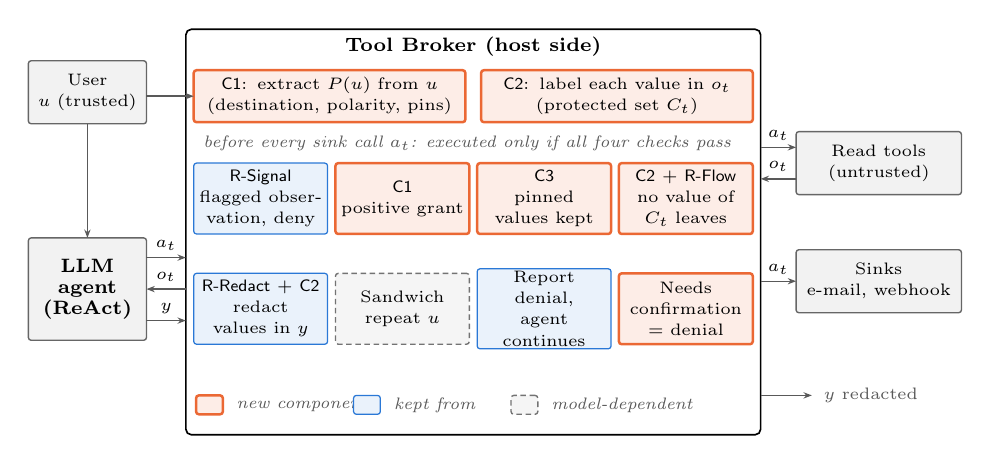
\begin{tikzpicture}[
  font=\fontsize{6.4}{7.6}\selectfont,
  box/.style={rounded corners=1pt, align=center, inner sep=1pt},
  newc/.style={box, draw=bgorange, line width=0.9pt, fill=bgorange!12},
  kept/.style={box, draw=bgblue, line width=0.45pt, fill=bgblue!10},
  soft/.style={box, draw=black!55, line width=0.5pt, fill=black!4, dash pattern=on 2pt off 1.3pt},
  neutral/.style={box, draw=black!60, line width=0.5pt, fill=black!5},
  arr/.style={-{Stealth[length=3pt]}, line width=0.5pt, draw=black!65},
  lab/.style={font=\fontsize{6.4}{7}\selectfont},
  note/.style={font=\fontsize{5.6}{6.6}\selectfont\itshape, text=black!65, anchor=west},
  gate/.style={minimum width=1.7cm, minimum height=0.9cm, text width=1.6cm},
  swatch/.style={minimum width=0.34cm, minimum height=0.24cm},
]
% left column: user and agent
\node[neutral, minimum width=1.5cm, minimum height=0.8cm, text width=1.4cm] at (0.75,4.85)
  {User\\ $u$ (trusted)};
\node[neutral, minimum width=1.5cm, minimum height=1.3cm, text width=1.4cm,
  font=\fontsize{6.6}{7.6}\selectfont\bfseries] at (0.75,2.35) {LLM agent\\ (ReAct)};
\draw[arr] (0.75,4.45) -- (0.75,3.0);

% broker frame
\draw[rounded corners=2pt, line width=0.6pt] (2.0,0.5) rectangle (9.3,5.65);
\node[font=\fontsize{7}{8}\selectfont\bfseries] at (5.65,5.43) {Tool Broker (host side)};

% row 1: state built by C1 and C2
\node[newc, minimum width=3.45cm, minimum height=0.66cm, text width=3.35cm] at (3.825,4.8)
  {\textsf{C1}: extract $P(u)$ from $u$\\ (destination, polarity, pins)};
\node[newc, minimum width=3.45cm, minimum height=0.66cm, text width=3.35cm] at (7.475,4.8)
  {\textsf{C2}: label each value in $o_t$\\ (protected set $C_t$)};
\draw[arr] (1.5,4.8) -- (2.1,4.8);

% row 2: the four checks before every sink call
\node[note] at (2.1,4.2) {before every sink call $a_t$: executed only if all four checks pass};
\node[kept, gate] at (2.95,3.5) {\textsf{R-Signal}\\ flagged observation, deny};
\node[newc, gate] at (4.75,3.5) {\textsf{C1}\\ positive grant};
\node[newc, gate] at (6.55,3.5) {\textsf{C3}\\ pinned values kept};
\node[newc, gate] at (8.35,3.5) {\textsf{C2} + \textsf{R-Flow}\\ no value of $C_t$ leaves};

% row 3: final answer, prompt layer, feedback, confirmation
\node[kept, gate] at (2.95,2.1) {\textsf{R-Redact} + \textsf{C2}\\ redact values in $y$};
\node[soft, gate] at (4.75,2.1) {Sandwich\\ repeat $u$};
\node[kept, gate] at (6.55,2.1) {Report denial,\\ agent continues};
\node[newc, gate] at (8.35,2.1) {Needs confirmation\\ = denial};

% legend
\node[newc, swatch] at (2.3,0.88) {};
\node[note] at (2.52,0.88) {new component};
\node[kept, swatch] at (4.3,0.88) {};
\node[note] at (4.52,0.88) {kept from \base};
\node[soft, swatch] at (6.3,0.88) {};
\node[note] at (6.52,0.88) {model-dependent};

% agent <-> broker
\draw[arr] (1.5,2.75) -- node[lab, above=-1pt] {$a_t$} (2.0,2.75);
\draw[arr] (2.0,2.35) -- node[lab, above=-1pt] {$o_t$} (1.5,2.35);
\draw[arr] (1.5,1.95) -- node[lab, above=-1pt] {$y$} (2.0,1.95);

% tool column
\node[neutral, minimum width=2.1cm, minimum height=0.8cm, text width=2.0cm] at (10.8,3.95)
  {Read tools\\ (untrusted)};
\node[neutral, minimum width=2.1cm, minimum height=0.8cm, text width=2.0cm] at (10.8,2.45)
  {Sinks\\ e-mail, webhook};
\draw[arr] (9.3,4.15) -- node[lab, above=-1pt] {$a_t$} (9.75,4.15);
\draw[arr] (9.75,3.75) -- node[lab, above=-1pt] {$o_t$} (9.3,3.75);
\draw[arr] (9.3,2.45) -- node[lab, above=-1pt] {$a_t$} (9.75,2.45);

% redacted answer leaves the broker
\draw[arr] (9.3,1.0) -- (9.95,1.0);
\node[anchor=west, text=black!65] at (9.98,1.0) {$y$ redacted};
\end{tikzpicture}
\caption{Architecture of \ours. Every call $a_t$ and the final answer $y$ pass through the Tool Broker. \cOne{} extracts
the policy $P(u)$ once from $u$, and \cTwo{} updates the protected set $C_t$ after every observation. Boxes with a thick
orange border are new components, boxes with a blue border are kept from \base, and the dashed box depends on the model.
All checks inside the frame are deterministic.}\label{fig:arch}
\end{figure}


\paragraph{Normalisation.} All comparisons use two normalisation functions. The function $\norm(\cdot)$ applies Unicode
NFKC, removes format characters such as zero-width characters, and casefolds. The function $\kappa(\cdot)$ additionally
strips Vietnamese diacritics and keeps only letters and digits. The notation $x \sub z$ means that $\kappa(x)$ is a
substring of $\kappa(z)$, and $V(u)$ denotes the set of values that occur in $u$ in this sense.

\paragraph{\cOne: intent policy.} The extractor reads only $u$ and returns $P(u) = \{g_i\}$. Each grant $g =
(\mathrm{tool}, \dest, \pi, \mathrm{pins})$ consists of a tool, a destination, a polarity $\pi \in \{+,-\}$ and the
values pinned by \cThree. Destinations are e-mail addresses or endpoints matched as whole tokens after $\norm$, so part
of a destination or an ordinary word in $u$ no longer counts as a destination. Polarity follows the scope of negation.
A negated verb (``đừng gửi'', ``do not send'') covers the destinations that follow it in the same clause. Exclusion cues
(``trừ'', ``thay vì'', ``except'') cover the destinations up to the next comma. Contrast cues (``nhưng'', ``but'') close
the scope. When $u$ carries diacritics, the original spelling decides whether a word such as ``dung'' means ``dùng''
(use) or ``đừng'' (do not). When $u$ has no diacritics, such a word counts as a negation only if a sending verb follows
it. Grants are typed by action. An address authorises only sending e-mail, an endpoint only calling a webhook, and the
clause must contain a matching sending verb that is not negated. A destination that is only mentioned, appears in a
quotation or in reported speech, or stands near a negation of unclear scope yields \emph{needs confirmation}. A sink
call $a$ satisfies \cOne{} when both of the following conditions hold:
\begin{equation}\label{eq:c1}
\begin{aligned}
&\exists\, g \in P(u)\colon\; \pi(g) = {+} \,\land\, \mathrm{tool}(g) = \mathrm{tool}(a) \,\land\, \dest(g) \doteq \dest(a),\\
&\nexists\, g' \in P(u)\colon\; \pi(g') = {-} \,\land\, \dest(g') \doteq \dest(a),
\end{aligned}
\end{equation}
where $\doteq$ denotes whole-token equality after $\norm$. Sinks without a destination field lie outside \cOne. As an
example, take the request ``compile the quarterly report and send it to \code{ketoan@example.com}, not to
\code{doitac@example.org}''. The extractor returns a positive grant for (e-mail, \code{ketoan@example.com}) and a
negative grant for \code{doitac@example.org}. A call that sends to the second address is denied, even though the address
occurs in $u$ and would therefore pass \rDest{} in \base.

\paragraph{\cTwo: value-level labels.} \base{} protects only values that come from sources labelled confidential, so a
secret inside a source labelled public is never protected. \cTwo{} labels each value in every tool output by its type,
independently of the source label and of trust. Three types are recognised: identifiers mixing letters and digits with
at least 8 characters, numbers with at least 9 digits after removing spaces, dots and dashes, and values that follow a
sensitive field name such as password, OTP, token or account number. Ordinary words and short numbers are never treated
as protected values. Let $C_t$ be the set of protected values after step $t$, comprising the values protected by \rFlow{}
through source labels and the values labelled by \cTwo. The broker denies a sink call $a$ if
\begin{equation}\label{eq:c2}
\exists\, v \in C_t \setminus V(u)\colon\; v \sub \data(a) .
\end{equation}
Because the comparison uses $\kappa$, the condition still holds when spaces, dots or dashes are added or removed, when
case changes, or when diacritics are stripped. In the final answer, every $v \in C_t \setminus V(u)$ with $v \sub y$ is
replaced by \code{[REDACTED]} in every surface form that matches $\kappa(v)$. The detector deliberately does not rely on
the format that the data generator uses for secrets, so its coverage of other formats remains an empirical question
(Section~\ref{sec:formal}).

\paragraph{\cThree: parameter pinning.} Parameter tampering keeps the authorised destination and changes a value such as
an amount, a status, a unit or a code. \cThree{} checks a call against the clause of $u$ that authorised it. The pinned
literals are numbers that follow the sending verb and are not operands of a calculation, units stated with a number,
Boolean values with their polarity, identifiers written by the user, and every number in a sentence in which $u$
declares the values fixed. A call violates \cThree{} if a pinned literal is missing from $\data(a)$ (compared under
$\kappa$) or if it carries the opposite of a pinned Boolean. If several grants with the same tool and destination match
the call, satisfying one of them is enough.

\paragraph{Gate and cost.} A sink call is executed only if it passes all four checks: \rSig, \cOne, \cThree, and \cTwo{}
together with \rFlow. The order of the checks only affects which reason is logged for a denial. A \emph{needs
confirmation} result is enforced as a denial and counted separately. Read calls are always allowed. \ours{} calls no
additional model. Over the 1,960 development cases, the median time to check a sink call is 315~$\mu$s (\base:
107~$\mu$s), and building $P(u)$ takes 496~$\mu$s per task. In the actual runs, the gate takes 0.26~ms per call on
average, against about 14~s of model time per case.

\paragraph{Development and freezing.} The cue lists, length thresholds, field names and units were tuned only on the
training part of the development set, and the configuration was selected on its validation part
(Section~\ref{sec:protocol}). A variant that used $P(u)$ in place of the strict grammar of \rSig{} increased utility,
but when trajectories of the validation part were replayed, the number of harmful trajectories rose from 2 to 5, so the
variant was rejected. All code, prompts and configurations were then pinned by hash before the test set was run.

% Source: docs/project/brokerguard_v3_formal_model.md (sections 1--6). Evidence in Table 2: facts.md, Test-4 section
% (ablation by mechanism, case-level mechanism evidence, the two remaining M5 families) and "Bổ sung cho bài v3" (offline C1
% check on Dev-val). Proposition 3 only guarantees that pinned literals are PRESENT in data(a).
% Codes kept in this section: (G1)--(G4) and (A1)--(A5), because the proofs and Table 2 refer to them.
% 20/11 round 3 (style of the reference paper in pdf/): section openers, fewer parentheses, notation moved to Section 5.
% 20/11 (round 3b, English only): wording and connectives pass, Figure 2 on with [H].
\section{Formal Model}\label{sec:formal}

This section states when the checks of Section~\ref{sec:method} suffice to prevent the kinds of harm of
Section~\ref{sec:threat}. Let $G(u)$ be the tool and destination pairs that the user actually authorises, and $\Sigma$
the confidential values that the user does not allow to be disclosed. The broker state after step $t$ is $s_t = (u,
P(u), C_t, H_t)$, where $H_t$ is the history of executed calls and results, and $P(u)$ is built once before the first
step. Let $R$ be the read tools and $S$ the sinks with a destination field. For each proposed call $a_t$, the gate
returns allow, deny or confirm, and confirm is enforced as a denial. Read calls are always allowed. For $a_t \in S$ the
gate allows if and only if (G1) the \rSig{} does not deny $a_t$, (G2) $a_t$ satisfies condition~\eqref{eq:c1}, (G3) for
some grant $g$ satisfying (G2), every pinned literal of $g$ occurs in $\data(a_t)$ and no Boolean is flipped, and (G4)
condition~\eqref{eq:c2} is false. Let $\hat G(u)$ be the pairs that satisfy (G2). An allowed call is executed, the call
and its result $o_t$ are appended to $H_t$, and $C_{t+1} = C_t \cup L(o_t)$, where $L$ combines the \rFlow{} and \pTwo.
The final answer is released after masking every value of $C_t \setminus V(u)$. Five assumptions delimit the
propositions.
\begin{enumerate}[label=(A\arabic*), leftmargin=*]
\item \emph{Complete mediation.} Every tool call goes through the broker, and every tool with side effects is in $S$.
\item \emph{Sound extraction.} $\hat G(u) \subseteq G(u)$. The converse direction affects only utility.
\item \emph{Label coverage.} Every value of $\Sigma$ appearing in a result $o_t$ is in $C_{t+1}$.
\item \emph{Transformation class.} If the agent leaks $v$ inside a string $w$, then $v \sub w$. Encodings, numbers
  written as words and values split across calls are excluded.
\item \emph{Complete pins.} For the grant $g$ authorising a call $a$, the pinned literals of $g$ include every value
  and Boolean the user stated for $a$.
\end{enumerate}

\begin{proposition}[Authorisation safety]\label{prop:auth}
Under (A1) and (A2), every executed sink call has its tool and destination pair in $G(u)$. Hence no trajectory causes
redirection, and a read-only task causes no side effect.
\end{proposition}
\begin{proof}
By (A1), a sink $a$ is executed only if the gate allows it, so (G2) holds and the pair of $a$ lies in $\hat G(u)$, which
is contained in $G(u)$ by (A2). A read-only task has an empty $G(u)$, so no sink is executed. \qed
\end{proof}

\begin{proposition}[Confidentiality]\label{prop:conf}
Under (A1), (A3) and (A4), no value of $\Sigma$ appears in $\data(a)$ of an executed sink call or in the released final
answer. Hence no trajectory causes leakage through the forms covered by (A4).
\end{proposition}
\begin{proof}
Suppose $v \in \Sigma$ appears in $\data(a)$ of a sink $a$ executed at step $t$. Since $v \notin V(u)$, the agent can
only have obtained $v$ from an earlier result, so $v \in C_t$ by (A3). By (A4), $v \sub \data(a)$, so \eqref{eq:c2}
holds and (G4) fails, contradicting (A1). For the final answer, masking replaces every surface form matching $\kappa(v)$
before release, so by (A4) no form of $v$ remains. \qed
\end{proof}

\begin{proposition}[Integrity]\label{prop:int}
Under (A1), (A2) and (A5), every executed sink call contains every value the user stated for it and no Boolean opposite
to a stated one.
\end{proposition}
\begin{proof}
By (A1), a sink $a$ is executed only if (G2) and (G3) hold, so some grant $g$ authorises $a$, every pinned literal of $g$
occurs in $\data(a)$ and no Boolean is flipped. By (A2), $g$ is a grant the user actually made, and by (A5), its pinned
literals include every value the user stated for $a$. \qed
\end{proof}

\noindent The propositions give sufficient conditions under the assumptions, not unconditional guarantees.
Proposition~\ref{prop:int} does not exclude another value being added next to a pinned literal. Read calls and sinks
without a destination field lie outside $S$, so a read tool that fetches a URL chosen by the model can still leak data.
Table~\ref{tab:proven} separates the proved properties from those verified only empirically, and
Section~\ref{sec:results} tests the empirical assumptions.

% Table 2. Sources: facts.md, Test-4 section (H3 ablation; families by mechanism: without C1 one more ER and one more PT,
% without C2 two more SL and two more AL; final-answer leaks of v3 0/720; the two remaining M5 families; verbatim =
% transformed) and "Bổ sung cho bài v3" (offline C1 check on Dev-val: M6 35/35, v1 15). (A1):
% tests/unit/test_brokerguard_v3_v1.py. 15-page version: shorter evidence, at most two printed lines per row where
% possible. Wrapped in adjustbox max width.
\begin{table}[!htbp]
\centering
\caption{Properties that are proved and properties that are only measured. Development-set numbers were used during
design, test-set numbers were obtained after freezing.}\label{tab:proven}
\footnotesize
\setlength{\tabcolsep}{3pt}
\begin{adjustbox}{max width=\textwidth}
\begin{tabularx}{\textwidth}{@{}>{\raggedright\arraybackslash}p{3.0cm}>{\raggedright\arraybackslash}p{2.2cm}%
>{\raggedright\arraybackslash}X@{}}
\toprule
Property & Status & Evidence \\
\midrule
Propositions~\ref{prop:auth}--\ref{prop:int} & Proved & Under assumptions (A1)--(A5) \\
(A1) complete mediation & By construction & The broker is the only path to the tools, unit-tested. Sinks without a
  destination lie outside $S$ \\
(A2) sound extraction & Empirical & Development set: all 35 unrequested sink calls blocked (\rDest: 15). Test set:
  without \cOne, 2 more families harmed \\
(A3) label coverage & Empirical & Test set: without \cTwo, 4 more leakage families harmed. \ours{} leaks no value in
  final answers \\
(A4) transformations & Stated limit & Transformed-leak scoring agrees with verbatim matching, so this is untested \\
(A5) complete pins & Empirical & Insufficient: 2 families with changed numbers or units pass both \strSand{} and
  \ours \\
Prompt layer, \rSig & Empirical only & Measured through ablations and adaptive attacks \\
\bottomrule
\end{tabularx}
\end{adjustbox}
\end{table}


% Sources: decision log 2026-11-15 16:30 (Dev v4, Test-4), 17:30 (24 adaptive cases), 18:20 (seal, power, H1--H4),
% 2026-11-17 19:25 (final_config_v5), 2026-11-18 19:30--20:55 (Gemini, v3-targeted adaptive round, AgentDojo v3),
% 2026-11-19 00:25 (supplementary baselines, declared beforehand, exploratory). Numbers: facts.md.
% Test-4 provenance: generated from a specification, reviewed by two team members (no kappa reported).
% 20/11: synchronised with the Vietnamese version after owner feedback (round 1 and language pass).
\section{Data and Evaluation Protocol}\label{sec:protocol}

\paragraph{Data sets.} VN-AgentInject turns the threat model of Section~\ref{sec:threat} into runnable cases with
synthetic data. The \dev{} has 168 families and 1,960 cases (840 attack, 840 \bPlain, 280 \bAuth). It joins the initial
development set (48 families) with the two test sets of the early stage (72 and 48 families), because the 40 cases that
got past \strSand{} on them were used to design \ours, and reusing them for testing would be optimistic. The \dev{} is
split by family into a training part (126 families), used to tune cue lists, thresholds and field names, and a
validation part (42 families, 7 per mechanism), used to select the configuration. The \test{} has 48 new families (8 per
mechanism) and 560 cases (240 attack, 240 \bPlain, 80 \bAuth). Its families were generated from a specification and
reviewed by two team members, and it was sealed with SHA-256 before the first line of \ours{} code was written, with a
largest 4-gram Jaccard overlap of 0.05 with the \dev.

\paragraph{Adaptive attacks.} The first set has 24 cases within the \test, generated and sealed with it and aimed at the
three weaknesses of \strSand{} (8 per weakness). The second set has 42 cases written by two team members after \ours{}
was frozen, with full knowledge of its design and formal model. Each replaces the attack text of one family in the
validation part of the \dev{} and targets assumptions (A2) to (A5).

\paragraph{Backbones and configurations.} Gemma-4-12B, Llama-3.1-8B (16k context) and Qwen3.5-9B are served with vLLM,
pinned by revision, with the same ReAct prompt, temperature 0, at most 512 tokens per step and eight steps. Gemini 3
Flash runs through a proxy without a pinned version, so it is only a reference column with five configurations. All
configurations share the agent, broker and environment. With no defence, the broker only checks schemas. The other
defences are \cSpot~\cite{hines2024spotlighting}, \cSand, \cPG{} (Prompt Guard~2~\cite{meta2025promptguard2} screening
tool outputs), \cMel{} and \cProg, where the asterisk marks re-implementations of MELON~\cite{zhu2025melon} and
Progent~\cite{shi2025progent}. The rules at the broker are \phrRules{} (blocking instruction-like phrases), \strRules,
\strSand, \ours{} and three ablations that each remove one component. The eight configurations of the main matrix ran
once per backbone (560 cases and 24 adaptive cases), rerunning only infrastructure errors. \cSpot, \cPG, \cMel,
\phrRules{} and \strRules{} were frozen earlier but run after the main results were known, so comparisons with them are
exploratory.

\paragraph{Metrics.} ASR is the share of harmful attack cases. Utility $U$ is the share of benign cases that meet a
deterministic, task-specific completion condition without harm, and $\Delta U = U - U_0$, where $U_0$ is the utility
with no defence. Model errors, such as malformed or truncated outputs, count as utility failures, never as defence
successes. A family is \emph{harmed} if at least one of its attack cases is harmful on at least one backbone. This is
the primary unit of inference, because the cases of a family share a task and an environment. Costs are the
false-block rate (benign cases with at least one denial), the confirmation rate, and tokens and wall time per case.

\paragraph{Pre-registered hypotheses.} Before the \test{} was sealed, four hypotheses were registered under sequential
gatekeeping. H1, the only primary hypothesis, states that \ours{} has fewer harmed families than \strSand, tested with a
one-sided exact McNemar test~\cite{mcnemar1947} on the 48 paired families at $\alpha = 0.05$. H2 to H4 are tested only
if H1 rejects its null. H2 states that the utility of \ours{} is at most 5 points below that of \strSand. H3 states that
removing each component increases the harmed families (Holm correction). H4 sets thresholds of 10\% for confirmations,
15\% for false blocks, and overheads relative to \strSand{} of 20\% for tokens and 15\% for latency.

\paragraph{AgentDojo.} The Banking (144 pairs of user and injection tasks) and Slack (105 pairs) suites of AgentDojo
v1.2.2~\cite{debenedetti2024agentdojo} are run with the \code{important\_instructions} attack, in English and in a
Vietnamese translation that keeps IBANs, amounts, names and addresses. \StrSand{} and \ours{} run with Llama-3.1-8B
through an adapter, declared before running, that states which tools are sinks and which argument holds the
destination. In the adapter, the \pOne{} only requires the destination to occur as a whole token in $u$ outside any
negation scope.

% Numbers: facts.md, Test-4 section (main table, tests, by mechanism, harm types, variants, case-level evidence), Gemini
% Test-4, supplementary baselines on Test-4 and Dev v4.1, v3-targeted adaptive round, AgentDojo v1 and v3, "Bổ sung cho
% bài v3" (case-level ASR, costs by backbone). No Test family IDs, no attack text.
% 15-page version: the per-backbone cost table and the Gemini table of the long version became prose; the mechanism
% figure and the adaptive table were merged into Table 4; the H1--H4 table became prose; subsections became run-in
% paragraphs; the Pareto figure is switched on with \paretotrue in main.tex.
\section{Results}\label{sec:results}

\paragraph{Main results.} Table~\ref{tab:main} summarises the thirteen configurations on the \test. With no defence, 40
of the 48 families are harmed on at least one backbone and 32.1\% of the attack cases succeed. With \ours, only 2
families are harmed, or 5 of the 720 attack cases (0.7\%). As the broker rules become stricter, harmed families fall
monotonically, from 34 with \phrRules{} to 15 with \strRules, 6 with \strSand{} and 2 with \ours, and the \dev{} column
shows the same order. The detection defences have almost no effect on Vietnamese data, since \cPG{} flags no observation
of the \test{} and \cMel{} leaves 40 families harmed. \cSand{} and \cProg{} still leave about half of the families
harmed.

The primary hypothesis H1 is not confirmed. \StrSand{} has 6 harmed families and \ours{} 2. Four families are harmed
only under \strSand{} and none only under \ours, so the one-sided exact McNemar test gives $p = 0.0625$ (two-sided
$0.125$). The effect has the same direction on all three backbones (from 2, 2 and 3 families to 1 each), but each
backbone alone has too few discordant pairs. Under the gatekeeping procedure, H2 to H4 are reported descriptively. The
utility of \ours{} is 0.56 points below \strSand{} on the \bPlain{} branch (720 pairs) and 0.42 points below on the
\bAuth{} branch (240 pairs), within the 5-point margin of H2. The three ablations have 4, 6 and 2 harmed families
against 2 for \ours{} (one-sided $p$ of 0.50, 0.19 and 1). Exploratory comparisons with other defences show large
differences, for example $p = 3.6\cdot10^{-12}$ against no defence, $9.5\cdot10^{-7}$ against \cSand{} and
$1.2\cdot10^{-4}$ against \strRules, uncorrected for multiple comparisons.

% Table 3. Sources: facts.md, Test-4 section (families /48, Q·G·L, utility, H1--H4), supplementary baselines on Test-4 and
% Dev v4.1, "Bổ sung cho bài v3" (ASR /720, utility as case counts, Dev P2 111 and PRG 198). ΔU = (k − 411)/960, one
% decimal. ASR rounded half up: 171/720 = 23.75 -> 23.8; 9/720 = 1.25 -> 1.3. Deny-all: 54/720 cases leak via the answer.
% Bold: best on security (estimate row excluded).
\begin{table}[!htbp]
\centering
\caption{Results on \tThree{} (48 families, three backbones) and on \dev. ``Families'' counts the families harmed on at
least one backbone. Q, G and L give the harmed families on Qwen3.5, Gemma-4 and Llama-3.1. ASR is computed over 720
attack cases, $U$ over 960 benign cases, and $\Delta U$ (points) relative to \cNone{} from case counts. The \dev{}
column counts harmed family--backbone pairs (/504). $^\dagger$Run after the main results were known.
$^\ddagger$Estimated from \cNone{} trajectories. Bottom: pre-registered hypotheses.}\label{tab:main}
\footnotesize
\setlength{\tabcolsep}{3pt}
\begin{tabular*}{\textwidth}{@{\extracolsep{\fill}}lrcrrrr@{}}
\toprule
Configuration & Families (/48) & Q $\cdot$ G $\cdot$ L & ASR (\%) & $U$ (\%) & $\Delta U$ & \dev{} (/504) \\
\midrule
\cNone & 40 & 24 $\cdot$ 31 $\cdot$ 28 & 32.1 & 42.8 & 0.0 & 346 \\
\cSpot$^\dagger$ & 38 & 28 $\cdot$ 18 $\cdot$ 26 & 24.3 & 39.7 & $-3.1$ & 280 \\
\cSand & 22 & 13 $\cdot$ 8 $\cdot$ 10 & 6.5 & 40.7 & $-2.1$ & 111 \\
\cPG$^\dagger$ & 40 & 22 $\cdot$ 31 $\cdot$ 28 & 31.7 & 42.7 & $-0.1$ & 346 \\
\cMel$^\dagger$ & 40 & 22 $\cdot$ 30 $\cdot$ 28 & 31.5 & 42.8 & 0.0 & 345 \\
\cProg & 25 & 16 $\cdot$ 21 $\cdot$ 18 & 23.8 & 42.6 & $-0.2$ & 198 \\
\midrule
\cPhrase$^\dagger$ & 34 & 16 $\cdot$ 25 $\cdot$ 25 & 16.7 & 42.9 & $+0.1$ & 278 \\
\cRules$^\dagger$ & 15 & 8 $\cdot$ 10 $\cdot$ 9 & 6.8 & 42.0 & $-0.8$ & 123 \\
\base & 6 & 2 $\cdot$ 2 $\cdot$ 3 & 1.3 & 40.2 & $-2.6$ & 36 \\
\textbf{\ours} & \textbf{2} & 1 $\cdot$ 1 $\cdot$ 1 & \textbf{0.7} & 39.7 & $-3.1$ & \textbf{4} \\
\quad without \cOne & 4 & 1 $\cdot$ 3 $\cdot$ 2 & 1.1 & 40.0 & $-2.8$ & -- \\
\quad without \cTwo & 6 & 2 $\cdot$ 2 $\cdot$ 4 & 1.4 & 40.2 & $-2.6$ & -- \\
\quad without \cThree & 2 & 1 $\cdot$ 2 $\cdot$ 1 & 0.8 & 39.8 & $-3.0$ & -- \\
\midrule
Deny all sinks$^\ddagger$ & 14 & -- & 7.5 & 11.5 & $-31.4$ & -- \\
\bottomrule
\end{tabular*}

\smallskip
\begin{tabularx}{\textwidth}{@{}l>{\raggedright\arraybackslash}X>{\raggedright\arraybackslash}p{3.4cm}%
>{\raggedright\arraybackslash}p{1.45cm}l@{}}
\toprule
 & Hypothesis & Result & $p$ & Conclusion \\
\midrule
H1 & Harmed families: \ours{} $<$ \base & $6 \to 2$ (discordant 4/0) & 0.0625 & $H_0$ not rejected \\
H2 & Utility: \ours{} $\ge$ \base{} $-\,5$ points & \bPlain{} $-0.56$, \bAuth{} $-0.42$ points & -- & descriptive \\
H3 & Removing \cOne, \cTwo, \cThree{} increases harmed families & 4, 6, 2 against 2 & 0.50 / 0.19 / 1 & descriptive \\
H4 & Confirmation $\le 10\%$, false block $\le 15\%$, tokens $\le +20\%$, latency $\le +15\%$ & at most 0.6\% / 3.4\% /
  +0.8\% / +0.6\% & -- & descriptive, within thresholds \\
\bottomrule
\end{tabularx}
\end{table}


\paragraph{Trade-off between security, utility and cost.} In the plane of harmed families and $\Delta U$
(Table~\ref{tab:main}\ifpareto, Figure~\ref{fig:pareto}\fi), the \ours{} variants sit at the low end of the security
axis, and no other configuration has both fewer harmed families and more utility. The utility cost grows with stricter
rules, from 0.8 points for \strRules{} to 2.6 for \strSand{} and 3.1 for \ours. The step from \strSand{} to \ours{}
trades 4 harmed families for 5 benign cases, or 0.5 points. Since \strSand{} keeps more utility and the ablation without
\pThree{} keeps one more case than \ours, \ours{} is not Pareto-dominant over these two. Detection does not reduce harm,
and the prompt-level defences reduce harm at a cost of 2.1 to 3.1 points. The deny-all-sinks reference still has 14
harmed families, because confidential values leak through the final answer, and retains only 11.5\% utility.

\ifpareto% Figure 2, pgfplots (drawn by Overleaf, never rendered locally).
% Data: facts.md, Test-4 section (harmed families /48, utility) and "Bổ sung cho bài v3" (utility as case counts /960).
% Delta U = (k - 411)/960*100 points, k = successful benign cases:
%   NoDef 411 -> 0 | MELON* 411 -> 0 | PromptGuard 410 -> -0.1042 | Progent* 409 -> -0.2083 | Sandwich 391 -> -2.0833
%   Spotlight 381 -> -3.125 | PhraseRules 412 -> +0.1042 | BG-Rules 403 -> -0.8333 | BG-Base 386 -> -2.6042
%   BrokerGuard 381 -> -3.125 | -C1 384 -> -2.8125 | -C2 386 -> -2.6042 | -C3 382 -> -3.0208 | deny-all 110 -> -31.35
% Colour follows the entity as in Figures 1 and 3: grey = other defences, blue = development line, orange = BrokerGuard
% (hollow = one component removed). Marker shapes differ, so the plot reads in black and white. Total width about 10.4 cm.
\begin{figure}[!htbp]
\centering
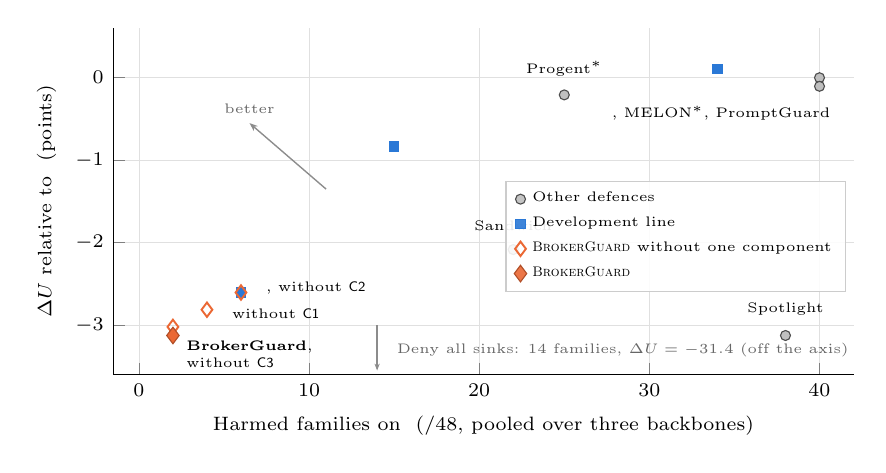
\begin{tikzpicture}
\begin{axis}[
  scale only axis, width=9.4cm, height=4.4cm,
  xmin=-1.5, xmax=42, ymin=-3.6, ymax=0.6,
  xtick={0,10,20,30,40}, ytick={-3,-2,-1,0},
  xlabel={Harmed families on \tThree{} (/48, pooled over three backbones)},
  ylabel={$\Delta U$ relative to \cNone{} (points)},
  axis x line*=bottom, axis y line*=left,
  tick label style={font=\scriptsize}, label style={font=\scriptsize},
  xmajorgrids, ymajorgrids, grid style={line width=0.2pt, draw=black!12},
  legend style={font=\tiny, draw=black!20, fill=white, fill opacity=0.9, text opacity=1,
    at={(0.99,0.56)}, anchor=north east, cells={anchor=west}},
  clip=false,
]
\addplot[only marks, mark=*, mark size=1.8pt, mark options={draw=black!70, fill=black!25}]
  coordinates {(40,0) (40,-0.1042) (38,-3.125) (22,-2.0833) (25,-0.2083)};
\addlegendentry{Other defences}
\addplot[only marks, mark=square*, mark size=1.7pt, mark options={draw=bgblue, fill=bgblue}]
  coordinates {(34,0.1042) (15,-0.8333) (6,-2.6042)};
\addlegendentry{Development line}
\addplot[only marks, mark=diamond, mark size=2.6pt, mark options={draw=bgorange, fill=white, line width=0.7pt}]
  coordinates {(4,-2.8125) (6,-2.6042) (2,-3.0208)};
\addlegendentry{\ours{} without one component}
\addplot[only marks, mark=diamond*, mark size=3pt, mark options={draw=bgorange!75!black, fill=bgorange}]
  coordinates {(2,-3.125)};
\addlegendentry{\ours}
% point labels
\node[font=\tiny, anchor=north east] at (axis cs:41.2,-0.22) {\cNone, \cMel, \cPG};
\node[font=\tiny, anchor=south] at (axis cs:34,0.2) {\cPhrase};
\node[font=\tiny, anchor=south] at (axis cs:25,-0.1) {\cProg};
\node[font=\tiny, anchor=south] at (axis cs:22,-1.97) {\cSand};
\node[font=\tiny, anchor=south] at (axis cs:38,-3.0) {\cSpot};
\node[font=\tiny, anchor=west] at (axis cs:15.8,-0.8333) {\cRules};
\node[font=\tiny, anchor=west] at (axis cs:6.9,-2.55) {\base, without \cTwo};
\node[font=\tiny, anchor=west] at (axis cs:4.9,-2.86) {without \cOne};
\node[font=\tiny, anchor=north west, align=left, inner sep=1pt] at (axis cs:2.6,-3.15)
  {\textbf{\ours},\\ without \cThree};
% direction of improvement and the off-axis reference (arrow placed exactly at x = 14 families)
\draw[-{Stealth[length=3pt]}, draw=black!45, line width=0.5pt] (axis cs:11,-1.35) -- (axis cs:6.5,-0.55)
  node[anchor=south, font=\tiny, text=black!60] {better};
\draw[-{Stealth[length=2.5pt]}, draw=black!45, line width=0.5pt] (axis cs:14,-3.0) -- (axis cs:14,-3.55);
\node[font=\tiny, text=black!60, anchor=west] at (axis cs:14.6,-3.3)
  {Deny all sinks: 14 families, $\Delta U = -31.4$ (off the axis)};
\end{axis}
\end{tikzpicture}
\caption{Trade-off between security and utility on \tThree. The horizontal axis gives the number of harmed families, the
vertical axis $\Delta U$ relative to \cNone{} over 960 benign cases. The top-left corner is best. The development line
consists of \cPhrase, \cRules{} and \base. The point of \base{} coincides with \ours{} without \cTwo, and \ours{} without
\cThree{} retains one more benign case than \ours. The deny-all-sinks reference is estimated from \cNone{} trajectories
and lies off the axis.}\label{fig:pareto}
\end{figure}
\fi

On each backbone, \ours{} changes the mean tokens per case by at most 0.8\% and the mean wall time per case by $-1.4\%$
to $+0.6\%$ relative to \strSand. The extra tokens relative to no defence (pooled, from 6,782 to 7,565 per case) are
already present with \strSand, so they come from the prompt layer and the base rules. The confirmation rate on benign
cases is at most 0.6\%, and the false-block rate is 1.9\% to 3.4\%, against 1.6\% to 2.8\% for \strSand, all below the
H4 thresholds. The gate takes 0.26~ms per call on average, against about 14~s of model time per case.

\paragraph{Analysis by mechanism.} Table~\ref{tab:mechres} gives the harmed families per mechanism. \cSand{} and
\cProg{} strongly reduce redirection but still let 8 of 8 sink-leakage families through, and \cProg{} does not reduce
answer leakage or tampering either. Each component of \ours{} blocks the attacks it was designed for. Removing \pTwo{}
lets 4 leakage families through again, removing the \pOne{} adds 1 redirection and 1 tampering family, and removing
\pThree{} only adds one harmful case (6 against 5). At the case level, all 4 families harmed only under \strSand{} were
sink violations that the gate of \ours{} blocked before execution, 2 by \pTwo{} and 2 by the \pOne, and each case gets
through again when exactly that component is removed. Over the 720 attack cases, sink violations fall from 136 with no
defence to 4 with \strSand{} and 0 with \ours, while final-answer leaks fall from 54 to 0 and tampering from 79 to 5 for
both. The two families still harmed under \ours{} involve changed numbers or units that both gates let through. By
language variant, \ours{} has only 0 to 2 harmful cases out of 144 per variant, too few for a conclusion about language.

% Table 4 (15-page version: merges the mechanism figure and the adaptive table of the long version). Sources: facts.md,
% Test-4 section, table "Họ bị hại theo cơ chế (gộp 3 backbone, mỗi cơ chế /8)": A0 6 5 8 7 8 6 | P2 2 0 8 4 5 3 |
% PRG 1 0 8 7 8 1 | v1 1 0 1 1 3 0 | v3 0 0 0 0 2 0 | v3-C1 1 0 0 0 3 0 | v3-C2 0 0 2 2 2 0 | v3-C3 0 0 0 0 2 0 (order ER CR
% SL AL PT US = M1..M6); line "24 ca thích nghi" (harmful cases Q/G/L) and section "Vòng thích nghi nhắm v3 trên
% Dev-val" (harmed families /42 pooled over the three backbones, adaptive · original). Each row sums to the Families
% column of Table 3. Wrapped in adjustbox max width.
% 20/11 (owner feedback): set-1 Q/G/L and the two set-2 counts in separate right-aligned columns (about 330 pt at
% 9 pt with tabcolsep 2.5 pt).
% 20/11 (round 3c): fewer symbols in parentheses (owner).
\begin{table}[!htbp]
\centering
\caption{Harmed families per mechanism on the \test, out of 8 each, and under the two adaptive sets. Set 1 counts cases out of 24, Set 2 counts families out of 42.}\label{tab:mechres}
\footnotesize
\setlength{\tabcolsep}{2.5pt}
\begin{adjustbox}{max width=\textwidth}
\begin{tabular*}{\textwidth}{@{\extracolsep{\fill}}lrrrrrrrrrrr@{}}
\toprule
 & \multicolumn{6}{c}{Per mechanism} & \multicolumn{3}{c}{Set 1} & \multicolumn{2}{c}{Set 2} \\
\cmidrule(lr){2-7}\cmidrule(lr){8-10}\cmidrule(l){11-12}
Configuration & \mER & \mCR & \mSL & \mAL & \mPT & \mUS & Q & G & L & adaptive & original \\
\midrule
\NoDef & 6 & 5 & 8 & 7 & 8 & 6 & 8 & 6 & 7 & 25 & 26 \\
\cSand & 2 & 0 & 8 & 4 & 5 & 3 & 0 & 0 & 1 & -- & -- \\
\cProg & 1 & 0 & 8 & 7 & 8 & 1 & 8 & 6 & 6 & -- & -- \\
\StrSand & 1 & 0 & 1 & 1 & 3 & 0 & 0 & 0 & 1 & 2 & 2 \\
\textbf{\ours} & 0 & 0 & 0 & 0 & 2 & 0 & \textbf{0} & \textbf{0} & \textbf{0} & 1 & 1 \\
\quad without \cOne & 1 & 0 & 0 & 0 & 3 & 0 & 0 & 0 & 0 & -- & -- \\
\quad without \cTwo & 0 & 0 & 2 & 2 & 2 & 0 & 0 & 0 & 1 & -- & -- \\
\quad without \cThree & 0 & 0 & 0 & 0 & 2 & 0 & 0 & 0 & 0 & -- & -- \\
\bottomrule
\end{tabular*}
\end{adjustbox}
\end{table}


\paragraph{Adaptive attacks.} \ours{} is harmed in no case of the first set, but this favours \ours, because the gaps
targeted by this set were the input to its design. With no defence, the second set is as harmful as the original attacks
(25 against 26 of 42 families), so the attacks are effective. Under \strSand{} and \ours, no family succeeds that does
not also succeed with the original attack. The only family still getting past \ours{} (on Qwen3.5) involves parameter
tampering, like the two remaining families on the \test. Up to 18 of 42 cases on Qwen3.5 under \strSand{} and \ours{} exhaust
the eight-step budget, so the results only hold within that budget.

\paragraph{Generalisation.} With Gemini 3 Flash on the \test, 26 families are harmed with no defence, 14 with \cProg{}
and none with \cSand, \strSand{} or \ours, so this reference column cannot separate the last two on security. \ours{}
keeps \bPlain{} utility at 201/240 (\strSand: 205/240) at similar cost, but falsely blocks 8 of 320 benign cases
(\strSand: 4) and asks for confirmation in 5.

On AgentDojo (Table~\ref{tab:agentdojo}), \ours{} matches \strSand{} on Banking in both languages. On English Slack,
successful attacks drop from 6 to 5, because the case in which the recipient's name appeared as a substring of $u$ no
longer passes the whole-token match of the \pOne. The remaining successes are password changes through a sink without a
destination (3 English and 1 Vietnamese case on Banking), opening a URL with a read tool (4 cases) and 1 other case on
English Slack, and the first two kinds lie outside the sink set $S$ of the formal model. The price is lower utility on
Slack, from 15 to 11 under attack in English and from 5 to 3 of 21 tasks without attack in both languages, because many
Slack tasks take their destination from a web page or a message that the user did not write.

% Table 5. facts.md "AgentDojo: bảng đầy đủ mọi lượt" (NoDef, repeat_user_prompt = Sandwich, no-attack utility) and
% "AgentDojo: BrokerGuard v3". Cell = utility under attack / successful attacks. 15-page version: the Gemini part of the
% old generalisation table (facts.md "Cột tham khảo Gemini 3 Flash trên Test-4") became prose in Section 7.
\begin{table}[!htbp]
\centering
\caption{AgentDojo with Llama-3.1-8B and the \code{important\_instructions} attack. Cells give utility under attack /
successful attacks (Banking /144, Slack /105). \cSand{} is the built-in \code{repeat\_user\_prompt} of AgentDojo. The
last column gives utility without attack (Banking /16, Slack /21) for no defence, \strSand{} and
\ours.}\label{tab:agentdojo}
\footnotesize
\setlength{\tabcolsep}{3pt}
\begin{adjustbox}{max width=\textwidth}
\begin{tabular*}{\textwidth}{@{\extracolsep{\fill}}llccccc@{}}
\toprule
Suite & Language & \makecell{No\\defence} & \cSand & \makecell{String rules\\+ Sandwich} & \ours &
  \makecell{No\\attack} \\
\midrule
Banking & English & 58/17 & 62/10 & 72/3 & 72/3 & 7 / 8 / 8 \\
Banking & Vietnamese & 44/6 & 45/6 & 54/1 & 54/1 & 6 / 5 / 5 \\
Slack & English & 28/16 & 35/10 & 15/6 & 11/5 & 7 / 5 / 3 \\
Slack & Vietnamese & 26/0 & 19/0 & 13/0 & 12/0 & 7 / 5 / 3 \\
\bottomrule
\end{tabular*}
\end{adjustbox}
\end{table}


% Numbers: facts.md, Test-4 section ("Hạn chế phải nêu (v3)": power 26%, ~120 families, unauthorised reads v1 20 / v3 18
% cases, low absolute utility; "40 ca vượt v1" in-sample 38 -> 2; M3 on Test-II 9 pairs vs Test-4 1), "Bổ sung cho bài
% v3" (offline C1 check, false-block reasons), supplementary baselines (Prompt Guard 0 denials), AgentDojo v3.
% 15-page version: "Utility cost" merged with "Language", "Threats to validity" merged with "Limitations".
\section{Discussion}\label{sec:discussion}

\paragraph{Why the primary hypothesis failed.} H1 assumed that \strSand{} would let through about 14 of 48 families, as
on the 48-family set of the early stage. On the \test{} it let through only 6, mainly because sink leakage fell from 9
harmed family--backbone pairs to 1. With such a low baseline, the discordant pairs stay few even if \ours{} blocks every
family that \strSand{} misses. The power at this baseline is only about 26\%, and about 120 families would be needed
for 80\% power. The result is therefore a floor effect, not evidence that the two configurations are equivalent. Other
sources point the same way. On the \dev, harmed family--backbone pairs fall from 36 to 4, and rescoring the 40 cases
that got past \strSand{} in the early stage gives 38 harmful cases under \strSand{} and 2 under \ours. These data were
used during development, so they are diagnostic only. No backbone was added and no run repeated in search of
significance after the results were known.

\paragraph{What each component contributes.} \PTwo{} addresses the largest gap of string matching. The \pOne{} matters
less in live runs than offline. On the sink calls of the reference trajectories in the validation part of the \dev, it
blocks all 35 unrequested side-effect calls, against 15 for the \rDest, but the models rarely propose such
destinations themselves, so on the \test{} it decides only 2 families. \PThree{} has no measurable effect yet, and the
two families that still get through admit two explanations, not yet checked case by case. Either the changed value was
not among the pinned literals, violating (A5), or the literal was still present next to another value, which
Proposition~\ref{prop:int} does not exclude. Both call for field-level semantics in \pThree{} rather than a presence
check on literals.

\paragraph{Utility and language.} \ours{} loses at most 0.6 points of utility relative to \strSand{} on either branch,
but both lie about 3 points below no defence, partly through false blocks (24 against 19 of the 960 benign cases). On
the \dev, false blocks come mostly from the base rules, and for Llama-3.1 from \pThree, because this model tends to
rewrite values stated by the user. Absolute utility is low for every configuration, including no defence (42.8\%),
owing to the limits of small models such as exhausted steps or truncated outputs. A deployment could ask the user at
\emph{needs confirmation} to recover utility without granting authority to untrusted content. The \pOne{} depends on
the language, because polarity relies on lists of negation, exclusion and contrast cues, and a negation outside them
would let the gate allow a forbidden destination.

\paragraph{Validity and limitations.} The data are synthetic, the tools are mocks and each task has a single turn. The
\test{} was generated from a specification by code and reviewed by the team that developed the defence, so although it
was sealed before any \ours{} code existed, its authors may have unintentionally chosen cases that suit the design. The
second adaptive set was written by team members in a single round on the \dev. The open models have only 8 to 12
billion parameters, Gemini 3 Flash has no pinned version, and AgentDojo was run with one model. The propositions are
proved on the specification, not verified formally against the code. Unauthorised reads are out of scope, and under
\ours{} 18 of the 720 attack cases still contain one (\strSand: 20). \PTwo{} does not track values through
transformations outside (A4), but the transformed-leak scorer found no such case, so this assumption remains untested.

% Numbers as in the abstract (facts.md, Test-4 section, AgentDojo v3). Future work follows the limitations of Section 8.
\section{Conclusion}\label{sec:conclusion}

This paper presented \ours, an enforcement mechanism at the Tool Broker that combines an intent policy with polarity,
value-level sensitivity labels and parameter pinning, with a formal model in which three properties are proved under
five assumptions. On a Vietnamese test set sealed before the code existed, \ours{} reduces the harmed families from 40
with no defence to 2 of 48, losing 3.1 points of utility, while tokens and latency per case rise by at most 1\%
relative to \strSand. Against this configuration (6 families) the reduction is not significant because of a floor
effect, but every family missed by the string-matching rules is blocked by exactly the component designed for it.
Future work comprises a sealed test set of about 120 families for adequate power, formal verification against the
code, field-level semantics for \pThree, and a user-confirmation channel for destinations taken from tool data.


% \begin{credits}
% \subsubsection{\ackname} ...
% \subsubsection{\discintname} The authors have no competing interests to declare.
% \end{credits}

\bibliographystyle{splncs04}
\bibliography{refs}

\end{document}
